\documentclass[letterpaper,8pt]{extarticle}
\usepackage[left=.65in,top=.65in,bottom=.65in,right=.65in]{geometry}
\usepackage{tikz}
\usetikzlibrary{arrows.meta, decorations.pathreplacing}
\definecolor{busred}{RGB}{200,40,40}
\definecolor{carblue}{RGB}{40,80,180}
\definecolor{corridorgreen}{RGB}{40,150,80}
\definecolor{Highlight}{HTML}{580F8B}
\pagestyle{empty}
\begin{document}
\begin{figure}[p]\centering
% generated by make_fig_tsp_actions.py -- edit the generator, not this file
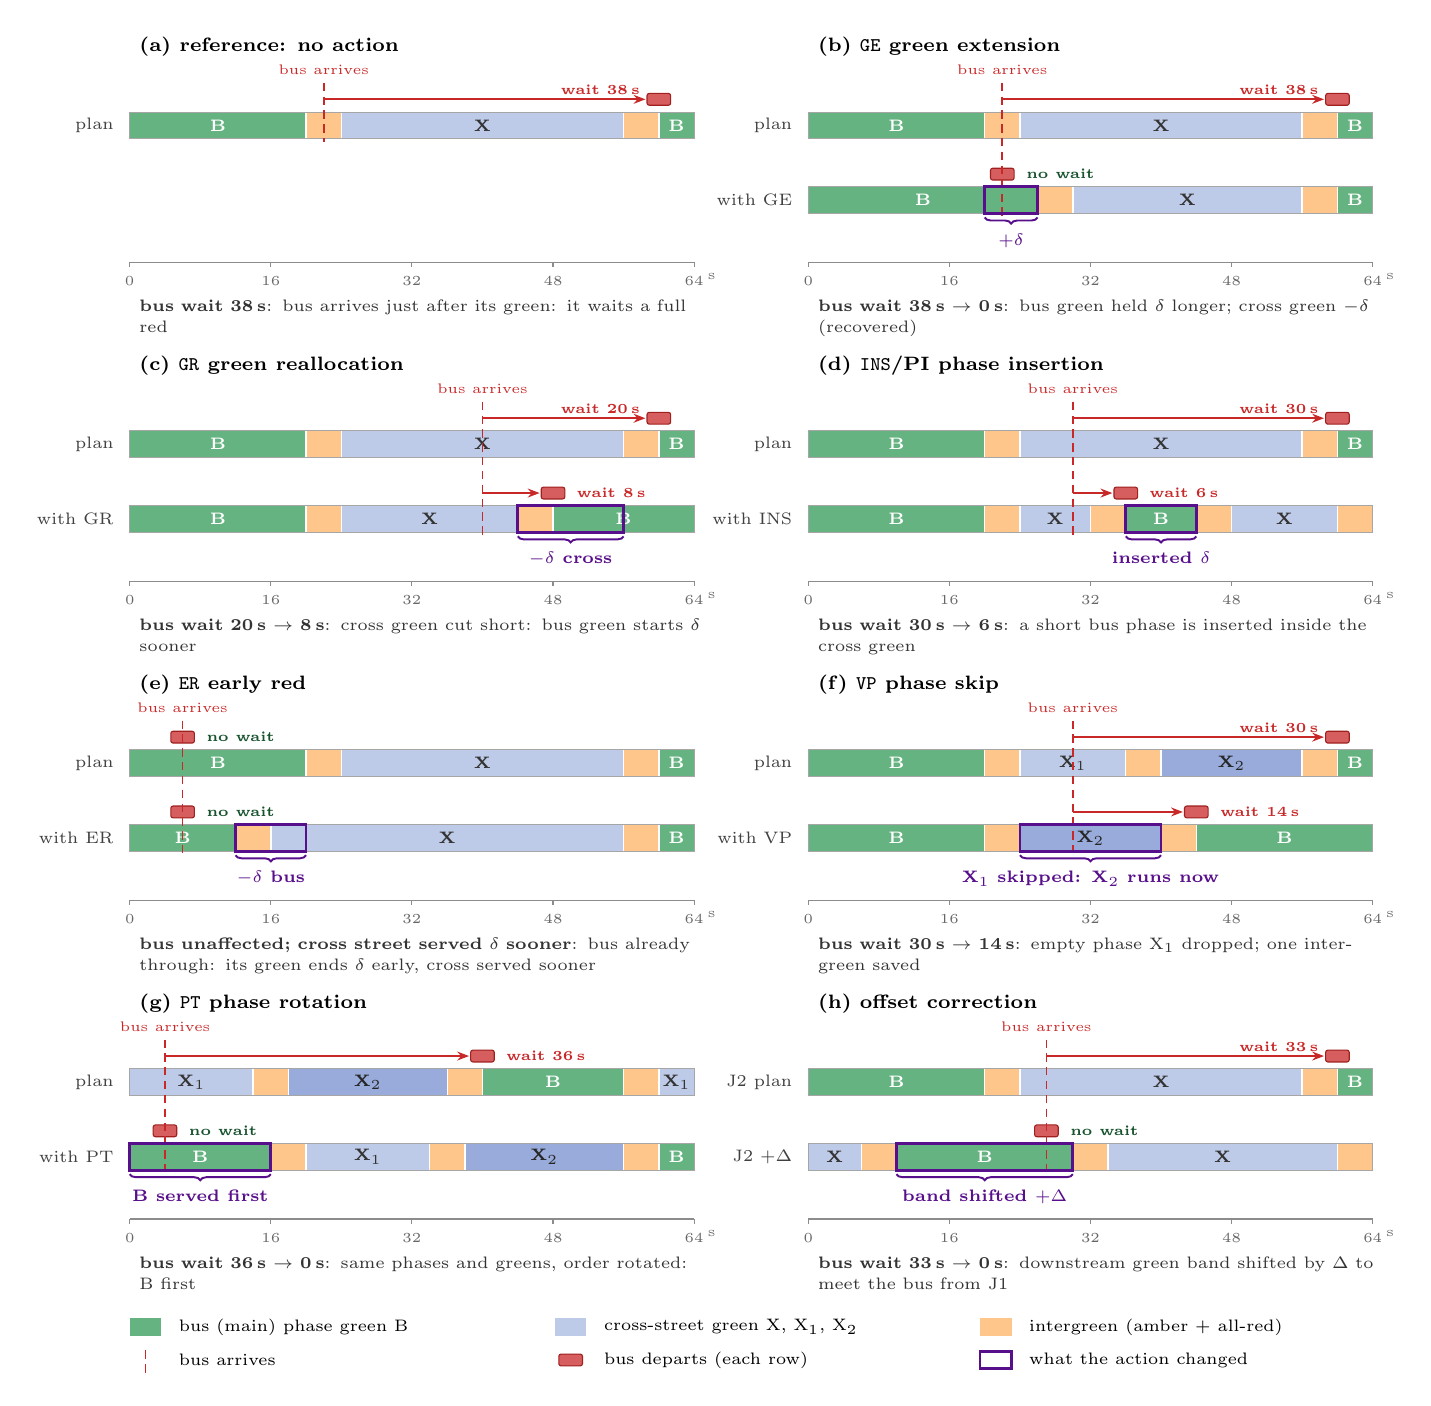
\begin{tikzpicture}[decoration={brace}]
\begin{scope}[shift={(0.000,0.000)}]
\node[anchor=west, font=\fontsize{7.5}{9}\selectfont\bfseries] at (0,2.12) {(a) reference: no action};
\node[anchor=east, font=\fontsize{6}{7}\selectfont, text=black!75] at (-0.08,1.120) {plan};
\fill[corridorgreen!72] (0.000,0.950) rectangle (2.240,1.290);
\draw[white, line width=0.5pt] (0.000,0.950) -- (0.000,1.290);
\node[font=\fontsize{6}{7}\selectfont\bfseries, text=white] at (1.120,1.120) {B};
\fill[orange!45] (2.240,0.950) rectangle (2.688,1.290);
\draw[white, line width=0.5pt] (2.240,0.950) -- (2.240,1.290);
\fill[carblue!30] (2.688,0.950) rectangle (6.272,1.290);
\draw[white, line width=0.5pt] (2.688,0.950) -- (2.688,1.290);
\node[font=\fontsize{6}{7}\selectfont\bfseries, text=black!80] at (4.480,1.120) {X};
\fill[orange!45] (6.272,0.950) rectangle (6.720,1.290);
\draw[white, line width=0.5pt] (6.272,0.950) -- (6.272,1.290);
\fill[corridorgreen!72] (6.720,0.950) rectangle (7.168,1.290);
\draw[white, line width=0.5pt] (6.720,0.950) -- (6.720,1.290);
\node[font=\fontsize{6}{7}\selectfont\bfseries, text=white] at (6.944,1.120) {B};
\draw[black!35, line width=0.3pt] (0,0.950) rectangle (7.168,1.290);
\draw[busred, line width=0.8pt, -{Stealth[length=1.5mm]}] (2.464,1.450) -- (6.550,1.450);
\node[draw=busred!80!black, fill=busred!75, rounded corners=0.8pt, minimum width=0.30cm, minimum height=0.15cm, inner sep=0pt] at (6.720,1.450) {};
\node[anchor=south east, font=\fontsize{5.5}{6}\selectfont\bfseries, text=busred, inner sep=1pt] at (6.520,1.470) {wait 38\,s};
\draw[busred, densely dashed, line width=0.6pt] (2.464,1.660) -- (2.464,0.910);
\node[font=\fontsize{5.5}{6}\selectfont, text=busred, anchor=south] at (2.464,1.640) {bus arrives};
\node[anchor=north west, align=left, text width=7.17cm, font=\fontsize{6.2}{7.4}\selectfont, text=black!80] at (0,-0.980) {\textbf{bus wait 38\,s}: bus arrives just after its green: it waits a full red};
\draw[black!45, line width=0.4pt] (0,-0.620) -- (7.168,-0.620);
\draw[black!45, line width=0.4pt] (0.000,-0.620) -- (0.000,-0.680) node[below, font=\fontsize{5.5}{6}\selectfont, text=black!60] {0};
\draw[black!45, line width=0.4pt] (1.792,-0.620) -- (1.792,-0.680) node[below, font=\fontsize{5.5}{6}\selectfont, text=black!60] {16};
\draw[black!45, line width=0.4pt] (3.584,-0.620) -- (3.584,-0.680) node[below, font=\fontsize{5.5}{6}\selectfont, text=black!60] {32};
\draw[black!45, line width=0.4pt] (5.376,-0.620) -- (5.376,-0.680) node[below, font=\fontsize{5.5}{6}\selectfont, text=black!60] {48};
\draw[black!45, line width=0.4pt] (7.168,-0.620) -- (7.168,-0.680) node[below, font=\fontsize{5.5}{6}\selectfont, text=black!60] {64};
\node[font=\fontsize{5.5}{6}\selectfont, text=black!60, anchor=west] at (7.218,-0.800) {s};
\end{scope}
\begin{scope}[shift={(8.618,0.000)}]
\node[anchor=west, font=\fontsize{7.5}{9}\selectfont\bfseries] at (0,2.12) {(b) \texttt{GE} green extension};
\node[anchor=east, font=\fontsize{6}{7}\selectfont, text=black!75] at (-0.08,1.120) {plan};
\fill[corridorgreen!72] (0.000,0.950) rectangle (2.240,1.290);
\draw[white, line width=0.5pt] (0.000,0.950) -- (0.000,1.290);
\node[font=\fontsize{6}{7}\selectfont\bfseries, text=white] at (1.120,1.120) {B};
\fill[orange!45] (2.240,0.950) rectangle (2.688,1.290);
\draw[white, line width=0.5pt] (2.240,0.950) -- (2.240,1.290);
\fill[carblue!30] (2.688,0.950) rectangle (6.272,1.290);
\draw[white, line width=0.5pt] (2.688,0.950) -- (2.688,1.290);
\node[font=\fontsize{6}{7}\selectfont\bfseries, text=black!80] at (4.480,1.120) {X};
\fill[orange!45] (6.272,0.950) rectangle (6.720,1.290);
\draw[white, line width=0.5pt] (6.272,0.950) -- (6.272,1.290);
\fill[corridorgreen!72] (6.720,0.950) rectangle (7.168,1.290);
\draw[white, line width=0.5pt] (6.720,0.950) -- (6.720,1.290);
\node[font=\fontsize{6}{7}\selectfont\bfseries, text=white] at (6.944,1.120) {B};
\draw[black!35, line width=0.3pt] (0,0.950) rectangle (7.168,1.290);
\draw[busred, line width=0.8pt, -{Stealth[length=1.5mm]}] (2.464,1.450) -- (6.550,1.450);
\node[draw=busred!80!black, fill=busred!75, rounded corners=0.8pt, minimum width=0.30cm, minimum height=0.15cm, inner sep=0pt] at (6.720,1.450) {};
\node[anchor=south east, font=\fontsize{5.5}{6}\selectfont\bfseries, text=busred, inner sep=1pt] at (6.520,1.470) {wait 38\,s};
\node[anchor=east, font=\fontsize{6}{7}\selectfont, text=black!75] at (-0.08,0.170) {with GE};
\fill[corridorgreen!72] (0.000,0.000) rectangle (2.912,0.340);
\draw[white, line width=0.5pt] (0.000,0.000) -- (0.000,0.340);
\node[font=\fontsize{6}{7}\selectfont\bfseries, text=white] at (1.456,0.170) {B};
\fill[orange!45] (2.912,0.000) rectangle (3.360,0.340);
\draw[white, line width=0.5pt] (2.912,0.000) -- (2.912,0.340);
\fill[carblue!30] (3.360,0.000) rectangle (6.272,0.340);
\draw[white, line width=0.5pt] (3.360,0.000) -- (3.360,0.340);
\node[font=\fontsize{6}{7}\selectfont\bfseries, text=black!80] at (4.816,0.170) {X};
\fill[orange!45] (6.272,0.000) rectangle (6.720,0.340);
\draw[white, line width=0.5pt] (6.272,0.000) -- (6.272,0.340);
\fill[corridorgreen!72] (6.720,0.000) rectangle (7.168,0.340);
\draw[white, line width=0.5pt] (6.720,0.000) -- (6.720,0.340);
\node[font=\fontsize{6}{7}\selectfont\bfseries, text=white] at (6.944,0.170) {B};
\draw[black!35, line width=0.3pt] (0,0.000) rectangle (7.168,0.340);
\node[draw=busred!80!black, fill=busred!75, rounded corners=0.8pt, minimum width=0.30cm, minimum height=0.15cm, inner sep=0pt] at (2.464,0.500) {};
\node[anchor=west, font=\fontsize{5.5}{6}\selectfont\bfseries, text=corridorgreen!55!black] at (2.644,0.500) {no wait};
\draw[busred, densely dashed, line width=0.6pt] (2.464,1.660) -- (2.464,-0.040);
\node[font=\fontsize{5.5}{6}\selectfont, text=busred, anchor=south] at (2.464,1.640) {bus arrives};
\draw[Highlight, line width=1.0pt] (2.240,0.000) rectangle (2.912,0.340);
\draw[Highlight, line width=0.7pt, decorate, decoration={brace, amplitude=2.2pt, mirror}] (2.240,-0.050) -- (2.912,-0.050);
\node[font=\fontsize{5.8}{6.5}\selectfont\bfseries, text=Highlight, anchor=north] at (2.576,-0.130) {$+\delta$};
\node[anchor=north west, align=left, text width=7.17cm, font=\fontsize{6.2}{7.4}\selectfont, text=black!80] at (0,-0.980) {\textbf{bus wait 38\,s $\rightarrow$ 0\,s}: bus green held $\delta$ longer; cross green $-\delta$ (recovered)};
\draw[black!45, line width=0.4pt] (0,-0.620) -- (7.168,-0.620);
\draw[black!45, line width=0.4pt] (0.000,-0.620) -- (0.000,-0.680) node[below, font=\fontsize{5.5}{6}\selectfont, text=black!60] {0};
\draw[black!45, line width=0.4pt] (1.792,-0.620) -- (1.792,-0.680) node[below, font=\fontsize{5.5}{6}\selectfont, text=black!60] {16};
\draw[black!45, line width=0.4pt] (3.584,-0.620) -- (3.584,-0.680) node[below, font=\fontsize{5.5}{6}\selectfont, text=black!60] {32};
\draw[black!45, line width=0.4pt] (5.376,-0.620) -- (5.376,-0.680) node[below, font=\fontsize{5.5}{6}\selectfont, text=black!60] {48};
\draw[black!45, line width=0.4pt] (7.168,-0.620) -- (7.168,-0.680) node[below, font=\fontsize{5.5}{6}\selectfont, text=black!60] {64};
\node[font=\fontsize{5.5}{6}\selectfont, text=black!60, anchor=west] at (7.218,-0.800) {s};
\end{scope}
\begin{scope}[shift={(0.000,-4.050)}]
\node[anchor=west, font=\fontsize{7.5}{9}\selectfont\bfseries] at (0,2.12) {(c) \texttt{GR} green reallocation};
\node[anchor=east, font=\fontsize{6}{7}\selectfont, text=black!75] at (-0.08,1.120) {plan};
\fill[corridorgreen!72] (0.000,0.950) rectangle (2.240,1.290);
\draw[white, line width=0.5pt] (0.000,0.950) -- (0.000,1.290);
\node[font=\fontsize{6}{7}\selectfont\bfseries, text=white] at (1.120,1.120) {B};
\fill[orange!45] (2.240,0.950) rectangle (2.688,1.290);
\draw[white, line width=0.5pt] (2.240,0.950) -- (2.240,1.290);
\fill[carblue!30] (2.688,0.950) rectangle (6.272,1.290);
\draw[white, line width=0.5pt] (2.688,0.950) -- (2.688,1.290);
\node[font=\fontsize{6}{7}\selectfont\bfseries, text=black!80] at (4.480,1.120) {X};
\fill[orange!45] (6.272,0.950) rectangle (6.720,1.290);
\draw[white, line width=0.5pt] (6.272,0.950) -- (6.272,1.290);
\fill[corridorgreen!72] (6.720,0.950) rectangle (7.168,1.290);
\draw[white, line width=0.5pt] (6.720,0.950) -- (6.720,1.290);
\node[font=\fontsize{6}{7}\selectfont\bfseries, text=white] at (6.944,1.120) {B};
\draw[black!35, line width=0.3pt] (0,0.950) rectangle (7.168,1.290);
\draw[busred, line width=0.8pt, -{Stealth[length=1.5mm]}] (4.480,1.450) -- (6.550,1.450);
\node[draw=busred!80!black, fill=busred!75, rounded corners=0.8pt, minimum width=0.30cm, minimum height=0.15cm, inner sep=0pt] at (6.720,1.450) {};
\node[anchor=south east, font=\fontsize{5.5}{6}\selectfont\bfseries, text=busred, inner sep=1pt] at (6.520,1.470) {wait 20\,s};
\node[anchor=east, font=\fontsize{6}{7}\selectfont, text=black!75] at (-0.08,0.170) {with GR};
\fill[corridorgreen!72] (0.000,0.000) rectangle (2.240,0.340);
\draw[white, line width=0.5pt] (0.000,0.000) -- (0.000,0.340);
\node[font=\fontsize{6}{7}\selectfont\bfseries, text=white] at (1.120,0.170) {B};
\fill[orange!45] (2.240,0.000) rectangle (2.688,0.340);
\draw[white, line width=0.5pt] (2.240,0.000) -- (2.240,0.340);
\fill[carblue!30] (2.688,0.000) rectangle (4.928,0.340);
\draw[white, line width=0.5pt] (2.688,0.000) -- (2.688,0.340);
\node[font=\fontsize{6}{7}\selectfont\bfseries, text=black!80] at (3.808,0.170) {X};
\fill[orange!45] (4.928,0.000) rectangle (5.376,0.340);
\draw[white, line width=0.5pt] (4.928,0.000) -- (4.928,0.340);
\fill[corridorgreen!72] (5.376,0.000) rectangle (7.168,0.340);
\draw[white, line width=0.5pt] (5.376,0.000) -- (5.376,0.340);
\node[font=\fontsize{6}{7}\selectfont\bfseries, text=white] at (6.272,0.170) {B};
\draw[black!35, line width=0.3pt] (0,0.000) rectangle (7.168,0.340);
\draw[busred, line width=0.8pt, -{Stealth[length=1.5mm]}] (4.480,0.500) -- (5.206,0.500);
\node[draw=busred!80!black, fill=busred!75, rounded corners=0.8pt, minimum width=0.30cm, minimum height=0.15cm, inner sep=0pt] at (5.376,0.500) {};
\node[anchor=west, font=\fontsize{5.5}{6}\selectfont\bfseries, text=busred] at (5.556,0.500) {wait 8\,s};
\draw[busred, densely dashed, line width=0.6pt] (4.480,1.660) -- (4.480,-0.040);
\node[font=\fontsize{5.5}{6}\selectfont, text=busred, anchor=south] at (4.480,1.640) {bus arrives};
\draw[Highlight, line width=1.0pt] (4.928,0.000) rectangle (6.272,0.340);
\draw[Highlight, line width=0.7pt, decorate, decoration={brace, amplitude=2.2pt, mirror}] (4.928,-0.050) -- (6.272,-0.050);
\node[font=\fontsize{5.8}{6.5}\selectfont\bfseries, text=Highlight, anchor=north] at (5.600,-0.130) {$-\delta$ cross};
\node[anchor=north west, align=left, text width=7.17cm, font=\fontsize{6.2}{7.4}\selectfont, text=black!80] at (0,-0.980) {\textbf{bus wait 20\,s $\rightarrow$ 8\,s}: cross green cut short: bus green starts $\delta$ sooner};
\draw[black!45, line width=0.4pt] (0,-0.620) -- (7.168,-0.620);
\draw[black!45, line width=0.4pt] (0.000,-0.620) -- (0.000,-0.680) node[below, font=\fontsize{5.5}{6}\selectfont, text=black!60] {0};
\draw[black!45, line width=0.4pt] (1.792,-0.620) -- (1.792,-0.680) node[below, font=\fontsize{5.5}{6}\selectfont, text=black!60] {16};
\draw[black!45, line width=0.4pt] (3.584,-0.620) -- (3.584,-0.680) node[below, font=\fontsize{5.5}{6}\selectfont, text=black!60] {32};
\draw[black!45, line width=0.4pt] (5.376,-0.620) -- (5.376,-0.680) node[below, font=\fontsize{5.5}{6}\selectfont, text=black!60] {48};
\draw[black!45, line width=0.4pt] (7.168,-0.620) -- (7.168,-0.680) node[below, font=\fontsize{5.5}{6}\selectfont, text=black!60] {64};
\node[font=\fontsize{5.5}{6}\selectfont, text=black!60, anchor=west] at (7.218,-0.800) {s};
\end{scope}
\begin{scope}[shift={(8.618,-4.050)}]
\node[anchor=west, font=\fontsize{7.5}{9}\selectfont\bfseries] at (0,2.12) {(d) \texttt{INS}/PI phase insertion};
\node[anchor=east, font=\fontsize{6}{7}\selectfont, text=black!75] at (-0.08,1.120) {plan};
\fill[corridorgreen!72] (0.000,0.950) rectangle (2.240,1.290);
\draw[white, line width=0.5pt] (0.000,0.950) -- (0.000,1.290);
\node[font=\fontsize{6}{7}\selectfont\bfseries, text=white] at (1.120,1.120) {B};
\fill[orange!45] (2.240,0.950) rectangle (2.688,1.290);
\draw[white, line width=0.5pt] (2.240,0.950) -- (2.240,1.290);
\fill[carblue!30] (2.688,0.950) rectangle (6.272,1.290);
\draw[white, line width=0.5pt] (2.688,0.950) -- (2.688,1.290);
\node[font=\fontsize{6}{7}\selectfont\bfseries, text=black!80] at (4.480,1.120) {X};
\fill[orange!45] (6.272,0.950) rectangle (6.720,1.290);
\draw[white, line width=0.5pt] (6.272,0.950) -- (6.272,1.290);
\fill[corridorgreen!72] (6.720,0.950) rectangle (7.168,1.290);
\draw[white, line width=0.5pt] (6.720,0.950) -- (6.720,1.290);
\node[font=\fontsize{6}{7}\selectfont\bfseries, text=white] at (6.944,1.120) {B};
\draw[black!35, line width=0.3pt] (0,0.950) rectangle (7.168,1.290);
\draw[busred, line width=0.8pt, -{Stealth[length=1.5mm]}] (3.360,1.450) -- (6.550,1.450);
\node[draw=busred!80!black, fill=busred!75, rounded corners=0.8pt, minimum width=0.30cm, minimum height=0.15cm, inner sep=0pt] at (6.720,1.450) {};
\node[anchor=south east, font=\fontsize{5.5}{6}\selectfont\bfseries, text=busred, inner sep=1pt] at (6.520,1.470) {wait 30\,s};
\node[anchor=east, font=\fontsize{6}{7}\selectfont, text=black!75] at (-0.08,0.170) {with INS};
\fill[corridorgreen!72] (0.000,0.000) rectangle (2.240,0.340);
\draw[white, line width=0.5pt] (0.000,0.000) -- (0.000,0.340);
\node[font=\fontsize{6}{7}\selectfont\bfseries, text=white] at (1.120,0.170) {B};
\fill[orange!45] (2.240,0.000) rectangle (2.688,0.340);
\draw[white, line width=0.5pt] (2.240,0.000) -- (2.240,0.340);
\fill[carblue!30] (2.688,0.000) rectangle (3.584,0.340);
\draw[white, line width=0.5pt] (2.688,0.000) -- (2.688,0.340);
\node[font=\fontsize{6}{7}\selectfont\bfseries, text=black!80] at (3.136,0.170) {X};
\fill[orange!45] (3.584,0.000) rectangle (4.032,0.340);
\draw[white, line width=0.5pt] (3.584,0.000) -- (3.584,0.340);
\fill[corridorgreen!72] (4.032,0.000) rectangle (4.928,0.340);
\draw[white, line width=0.5pt] (4.032,0.000) -- (4.032,0.340);
\node[font=\fontsize{6}{7}\selectfont\bfseries, text=white] at (4.480,0.170) {B};
\fill[orange!45] (4.928,0.000) rectangle (5.376,0.340);
\draw[white, line width=0.5pt] (4.928,0.000) -- (4.928,0.340);
\fill[carblue!30] (5.376,0.000) rectangle (6.720,0.340);
\draw[white, line width=0.5pt] (5.376,0.000) -- (5.376,0.340);
\node[font=\fontsize{6}{7}\selectfont\bfseries, text=black!80] at (6.048,0.170) {X};
\fill[orange!45] (6.720,0.000) rectangle (7.168,0.340);
\draw[white, line width=0.5pt] (6.720,0.000) -- (6.720,0.340);
\draw[black!35, line width=0.3pt] (0,0.000) rectangle (7.168,0.340);
\draw[busred, line width=0.8pt, -{Stealth[length=1.5mm]}] (3.360,0.500) -- (3.862,0.500);
\node[draw=busred!80!black, fill=busred!75, rounded corners=0.8pt, minimum width=0.30cm, minimum height=0.15cm, inner sep=0pt] at (4.032,0.500) {};
\node[anchor=west, font=\fontsize{5.5}{6}\selectfont\bfseries, text=busred] at (4.212,0.500) {wait 6\,s};
\draw[busred, densely dashed, line width=0.6pt] (3.360,1.660) -- (3.360,-0.040);
\node[font=\fontsize{5.5}{6}\selectfont, text=busred, anchor=south] at (3.360,1.640) {bus arrives};
\draw[Highlight, line width=1.0pt] (4.032,0.000) rectangle (4.928,0.340);
\draw[Highlight, line width=0.7pt, decorate, decoration={brace, amplitude=2.2pt, mirror}] (4.032,-0.050) -- (4.928,-0.050);
\node[font=\fontsize{5.8}{6.5}\selectfont\bfseries, text=Highlight, anchor=north] at (4.480,-0.130) {inserted $\delta$};
\node[anchor=north west, align=left, text width=7.17cm, font=\fontsize{6.2}{7.4}\selectfont, text=black!80] at (0,-0.980) {\textbf{bus wait 30\,s $\rightarrow$ 6\,s}: a short bus phase is inserted inside the cross green};
\draw[black!45, line width=0.4pt] (0,-0.620) -- (7.168,-0.620);
\draw[black!45, line width=0.4pt] (0.000,-0.620) -- (0.000,-0.680) node[below, font=\fontsize{5.5}{6}\selectfont, text=black!60] {0};
\draw[black!45, line width=0.4pt] (1.792,-0.620) -- (1.792,-0.680) node[below, font=\fontsize{5.5}{6}\selectfont, text=black!60] {16};
\draw[black!45, line width=0.4pt] (3.584,-0.620) -- (3.584,-0.680) node[below, font=\fontsize{5.5}{6}\selectfont, text=black!60] {32};
\draw[black!45, line width=0.4pt] (5.376,-0.620) -- (5.376,-0.680) node[below, font=\fontsize{5.5}{6}\selectfont, text=black!60] {48};
\draw[black!45, line width=0.4pt] (7.168,-0.620) -- (7.168,-0.680) node[below, font=\fontsize{5.5}{6}\selectfont, text=black!60] {64};
\node[font=\fontsize{5.5}{6}\selectfont, text=black!60, anchor=west] at (7.218,-0.800) {s};
\end{scope}
\begin{scope}[shift={(0.000,-8.100)}]
\node[anchor=west, font=\fontsize{7.5}{9}\selectfont\bfseries] at (0,2.12) {(e) \texttt{ER} early red};
\node[anchor=east, font=\fontsize{6}{7}\selectfont, text=black!75] at (-0.08,1.120) {plan};
\fill[corridorgreen!72] (0.000,0.950) rectangle (2.240,1.290);
\draw[white, line width=0.5pt] (0.000,0.950) -- (0.000,1.290);
\node[font=\fontsize{6}{7}\selectfont\bfseries, text=white] at (1.120,1.120) {B};
\fill[orange!45] (2.240,0.950) rectangle (2.688,1.290);
\draw[white, line width=0.5pt] (2.240,0.950) -- (2.240,1.290);
\fill[carblue!30] (2.688,0.950) rectangle (6.272,1.290);
\draw[white, line width=0.5pt] (2.688,0.950) -- (2.688,1.290);
\node[font=\fontsize{6}{7}\selectfont\bfseries, text=black!80] at (4.480,1.120) {X};
\fill[orange!45] (6.272,0.950) rectangle (6.720,1.290);
\draw[white, line width=0.5pt] (6.272,0.950) -- (6.272,1.290);
\fill[corridorgreen!72] (6.720,0.950) rectangle (7.168,1.290);
\draw[white, line width=0.5pt] (6.720,0.950) -- (6.720,1.290);
\node[font=\fontsize{6}{7}\selectfont\bfseries, text=white] at (6.944,1.120) {B};
\draw[black!35, line width=0.3pt] (0,0.950) rectangle (7.168,1.290);
\node[draw=busred!80!black, fill=busred!75, rounded corners=0.8pt, minimum width=0.30cm, minimum height=0.15cm, inner sep=0pt] at (0.672,1.450) {};
\node[anchor=west, font=\fontsize{5.5}{6}\selectfont\bfseries, text=corridorgreen!55!black] at (0.852,1.450) {no wait};
\node[anchor=east, font=\fontsize{6}{7}\selectfont, text=black!75] at (-0.08,0.170) {with ER};
\fill[corridorgreen!72] (0.000,0.000) rectangle (1.344,0.340);
\draw[white, line width=0.5pt] (0.000,0.000) -- (0.000,0.340);
\node[font=\fontsize{6}{7}\selectfont\bfseries, text=white] at (0.672,0.170) {B};
\fill[orange!45] (1.344,0.000) rectangle (1.792,0.340);
\draw[white, line width=0.5pt] (1.344,0.000) -- (1.344,0.340);
\fill[carblue!30] (1.792,0.000) rectangle (6.272,0.340);
\draw[white, line width=0.5pt] (1.792,0.000) -- (1.792,0.340);
\node[font=\fontsize{6}{7}\selectfont\bfseries, text=black!80] at (4.032,0.170) {X};
\fill[orange!45] (6.272,0.000) rectangle (6.720,0.340);
\draw[white, line width=0.5pt] (6.272,0.000) -- (6.272,0.340);
\fill[corridorgreen!72] (6.720,0.000) rectangle (7.168,0.340);
\draw[white, line width=0.5pt] (6.720,0.000) -- (6.720,0.340);
\node[font=\fontsize{6}{7}\selectfont\bfseries, text=white] at (6.944,0.170) {B};
\draw[black!35, line width=0.3pt] (0,0.000) rectangle (7.168,0.340);
\node[draw=busred!80!black, fill=busred!75, rounded corners=0.8pt, minimum width=0.30cm, minimum height=0.15cm, inner sep=0pt] at (0.672,0.500) {};
\node[anchor=west, font=\fontsize{5.5}{6}\selectfont\bfseries, text=corridorgreen!55!black] at (0.852,0.500) {no wait};
\draw[busred, densely dashed, line width=0.6pt] (0.672,1.660) -- (0.672,-0.040);
\node[font=\fontsize{5.5}{6}\selectfont, text=busred, anchor=south] at (0.672,1.640) {bus arrives};
\draw[Highlight, line width=1.0pt] (1.344,0.000) rectangle (2.240,0.340);
\draw[Highlight, line width=0.7pt, decorate, decoration={brace, amplitude=2.2pt, mirror}] (1.344,-0.050) -- (2.240,-0.050);
\node[font=\fontsize{5.8}{6.5}\selectfont\bfseries, text=Highlight, anchor=north] at (1.792,-0.130) {$-\delta$ bus};
\node[anchor=north west, align=left, text width=7.17cm, font=\fontsize{6.2}{7.4}\selectfont, text=black!80] at (0,-0.980) {\textbf{bus unaffected; cross street served $\delta$ sooner}: bus already through: its green ends $\delta$ early, cross served sooner};
\draw[black!45, line width=0.4pt] (0,-0.620) -- (7.168,-0.620);
\draw[black!45, line width=0.4pt] (0.000,-0.620) -- (0.000,-0.680) node[below, font=\fontsize{5.5}{6}\selectfont, text=black!60] {0};
\draw[black!45, line width=0.4pt] (1.792,-0.620) -- (1.792,-0.680) node[below, font=\fontsize{5.5}{6}\selectfont, text=black!60] {16};
\draw[black!45, line width=0.4pt] (3.584,-0.620) -- (3.584,-0.680) node[below, font=\fontsize{5.5}{6}\selectfont, text=black!60] {32};
\draw[black!45, line width=0.4pt] (5.376,-0.620) -- (5.376,-0.680) node[below, font=\fontsize{5.5}{6}\selectfont, text=black!60] {48};
\draw[black!45, line width=0.4pt] (7.168,-0.620) -- (7.168,-0.680) node[below, font=\fontsize{5.5}{6}\selectfont, text=black!60] {64};
\node[font=\fontsize{5.5}{6}\selectfont, text=black!60, anchor=west] at (7.218,-0.800) {s};
\end{scope}
\begin{scope}[shift={(8.618,-8.100)}]
\node[anchor=west, font=\fontsize{7.5}{9}\selectfont\bfseries] at (0,2.12) {(f) \texttt{VP} phase skip};
\node[anchor=east, font=\fontsize{6}{7}\selectfont, text=black!75] at (-0.08,1.120) {plan};
\fill[corridorgreen!72] (0.000,0.950) rectangle (2.240,1.290);
\draw[white, line width=0.5pt] (0.000,0.950) -- (0.000,1.290);
\node[font=\fontsize{6}{7}\selectfont\bfseries, text=white] at (1.120,1.120) {B};
\fill[orange!45] (2.240,0.950) rectangle (2.688,1.290);
\draw[white, line width=0.5pt] (2.240,0.950) -- (2.240,1.290);
\fill[carblue!30] (2.688,0.950) rectangle (4.032,1.290);
\draw[white, line width=0.5pt] (2.688,0.950) -- (2.688,1.290);
\node[font=\fontsize{6}{7}\selectfont\bfseries, text=black!80] at (3.360,1.120) {X$_1$};
\fill[orange!45] (4.032,0.950) rectangle (4.480,1.290);
\draw[white, line width=0.5pt] (4.032,0.950) -- (4.032,1.290);
\fill[carblue!48] (4.480,0.950) rectangle (6.272,1.290);
\draw[white, line width=0.5pt] (4.480,0.950) -- (4.480,1.290);
\node[font=\fontsize{6}{7}\selectfont\bfseries, text=black!85] at (5.376,1.120) {X$_2$};
\fill[orange!45] (6.272,0.950) rectangle (6.720,1.290);
\draw[white, line width=0.5pt] (6.272,0.950) -- (6.272,1.290);
\fill[corridorgreen!72] (6.720,0.950) rectangle (7.168,1.290);
\draw[white, line width=0.5pt] (6.720,0.950) -- (6.720,1.290);
\node[font=\fontsize{6}{7}\selectfont\bfseries, text=white] at (6.944,1.120) {B};
\draw[black!35, line width=0.3pt] (0,0.950) rectangle (7.168,1.290);
\draw[busred, line width=0.8pt, -{Stealth[length=1.5mm]}] (3.360,1.450) -- (6.550,1.450);
\node[draw=busred!80!black, fill=busred!75, rounded corners=0.8pt, minimum width=0.30cm, minimum height=0.15cm, inner sep=0pt] at (6.720,1.450) {};
\node[anchor=south east, font=\fontsize{5.5}{6}\selectfont\bfseries, text=busred, inner sep=1pt] at (6.520,1.470) {wait 30\,s};
\node[anchor=east, font=\fontsize{6}{7}\selectfont, text=black!75] at (-0.08,0.170) {with VP};
\fill[corridorgreen!72] (0.000,0.000) rectangle (2.240,0.340);
\draw[white, line width=0.5pt] (0.000,0.000) -- (0.000,0.340);
\node[font=\fontsize{6}{7}\selectfont\bfseries, text=white] at (1.120,0.170) {B};
\fill[orange!45] (2.240,0.000) rectangle (2.688,0.340);
\draw[white, line width=0.5pt] (2.240,0.000) -- (2.240,0.340);
\fill[carblue!48] (2.688,0.000) rectangle (4.480,0.340);
\draw[white, line width=0.5pt] (2.688,0.000) -- (2.688,0.340);
\node[font=\fontsize{6}{7}\selectfont\bfseries, text=black!85] at (3.584,0.170) {X$_2$};
\fill[orange!45] (4.480,0.000) rectangle (4.928,0.340);
\draw[white, line width=0.5pt] (4.480,0.000) -- (4.480,0.340);
\fill[corridorgreen!72] (4.928,0.000) rectangle (7.168,0.340);
\draw[white, line width=0.5pt] (4.928,0.000) -- (4.928,0.340);
\node[font=\fontsize{6}{7}\selectfont\bfseries, text=white] at (6.048,0.170) {B};
\draw[black!35, line width=0.3pt] (0,0.000) rectangle (7.168,0.340);
\draw[busred, line width=0.8pt, -{Stealth[length=1.5mm]}] (3.360,0.500) -- (4.758,0.500);
\node[draw=busred!80!black, fill=busred!75, rounded corners=0.8pt, minimum width=0.30cm, minimum height=0.15cm, inner sep=0pt] at (4.928,0.500) {};
\node[anchor=west, font=\fontsize{5.5}{6}\selectfont\bfseries, text=busred] at (5.108,0.500) {wait 14\,s};
\draw[busred, densely dashed, line width=0.6pt] (3.360,1.660) -- (3.360,-0.040);
\node[font=\fontsize{5.5}{6}\selectfont, text=busred, anchor=south] at (3.360,1.640) {bus arrives};
\draw[Highlight, line width=1.0pt] (2.688,0.000) rectangle (4.480,0.340);
\draw[Highlight, line width=0.7pt, decorate, decoration={brace, amplitude=2.2pt, mirror}] (2.688,-0.050) -- (4.480,-0.050);
\node[font=\fontsize{5.8}{6.5}\selectfont\bfseries, text=Highlight, anchor=north] at (3.584,-0.130) {X$_1$ skipped: X$_2$ runs now};
\node[anchor=north west, align=left, text width=7.17cm, font=\fontsize{6.2}{7.4}\selectfont, text=black!80] at (0,-0.980) {\textbf{bus wait 30\,s $\rightarrow$ 14\,s}: empty phase X$_1$ dropped; one intergreen saved};
\draw[black!45, line width=0.4pt] (0,-0.620) -- (7.168,-0.620);
\draw[black!45, line width=0.4pt] (0.000,-0.620) -- (0.000,-0.680) node[below, font=\fontsize{5.5}{6}\selectfont, text=black!60] {0};
\draw[black!45, line width=0.4pt] (1.792,-0.620) -- (1.792,-0.680) node[below, font=\fontsize{5.5}{6}\selectfont, text=black!60] {16};
\draw[black!45, line width=0.4pt] (3.584,-0.620) -- (3.584,-0.680) node[below, font=\fontsize{5.5}{6}\selectfont, text=black!60] {32};
\draw[black!45, line width=0.4pt] (5.376,-0.620) -- (5.376,-0.680) node[below, font=\fontsize{5.5}{6}\selectfont, text=black!60] {48};
\draw[black!45, line width=0.4pt] (7.168,-0.620) -- (7.168,-0.680) node[below, font=\fontsize{5.5}{6}\selectfont, text=black!60] {64};
\node[font=\fontsize{5.5}{6}\selectfont, text=black!60, anchor=west] at (7.218,-0.800) {s};
\end{scope}
\begin{scope}[shift={(0.000,-12.150)}]
\node[anchor=west, font=\fontsize{7.5}{9}\selectfont\bfseries] at (0,2.12) {(g) \texttt{PT} phase rotation};
\node[anchor=east, font=\fontsize{6}{7}\selectfont, text=black!75] at (-0.08,1.120) {plan};
\fill[carblue!30] (0.000,0.950) rectangle (1.568,1.290);
\draw[white, line width=0.5pt] (0.000,0.950) -- (0.000,1.290);
\node[font=\fontsize{6}{7}\selectfont\bfseries, text=black!80] at (0.784,1.120) {X$_1$};
\fill[orange!45] (1.568,0.950) rectangle (2.016,1.290);
\draw[white, line width=0.5pt] (1.568,0.950) -- (1.568,1.290);
\fill[carblue!48] (2.016,0.950) rectangle (4.032,1.290);
\draw[white, line width=0.5pt] (2.016,0.950) -- (2.016,1.290);
\node[font=\fontsize{6}{7}\selectfont\bfseries, text=black!85] at (3.024,1.120) {X$_2$};
\fill[orange!45] (4.032,0.950) rectangle (4.480,1.290);
\draw[white, line width=0.5pt] (4.032,0.950) -- (4.032,1.290);
\fill[corridorgreen!72] (4.480,0.950) rectangle (6.272,1.290);
\draw[white, line width=0.5pt] (4.480,0.950) -- (4.480,1.290);
\node[font=\fontsize{6}{7}\selectfont\bfseries, text=white] at (5.376,1.120) {B};
\fill[orange!45] (6.272,0.950) rectangle (6.720,1.290);
\draw[white, line width=0.5pt] (6.272,0.950) -- (6.272,1.290);
\fill[carblue!30] (6.720,0.950) rectangle (7.168,1.290);
\draw[white, line width=0.5pt] (6.720,0.950) -- (6.720,1.290);
\node[font=\fontsize{6}{7}\selectfont\bfseries, text=black!80] at (6.944,1.120) {X$_1$};
\draw[black!35, line width=0.3pt] (0,0.950) rectangle (7.168,1.290);
\draw[busred, line width=0.8pt, -{Stealth[length=1.5mm]}] (0.448,1.450) -- (4.310,1.450);
\node[draw=busred!80!black, fill=busred!75, rounded corners=0.8pt, minimum width=0.30cm, minimum height=0.15cm, inner sep=0pt] at (4.480,1.450) {};
\node[anchor=west, font=\fontsize{5.5}{6}\selectfont\bfseries, text=busred] at (4.660,1.450) {wait 36\,s};
\node[anchor=east, font=\fontsize{6}{7}\selectfont, text=black!75] at (-0.08,0.170) {with PT};
\fill[corridorgreen!72] (0.000,0.000) rectangle (1.792,0.340);
\draw[white, line width=0.5pt] (0.000,0.000) -- (0.000,0.340);
\node[font=\fontsize{6}{7}\selectfont\bfseries, text=white] at (0.896,0.170) {B};
\fill[orange!45] (1.792,0.000) rectangle (2.240,0.340);
\draw[white, line width=0.5pt] (1.792,0.000) -- (1.792,0.340);
\fill[carblue!30] (2.240,0.000) rectangle (3.808,0.340);
\draw[white, line width=0.5pt] (2.240,0.000) -- (2.240,0.340);
\node[font=\fontsize{6}{7}\selectfont\bfseries, text=black!80] at (3.024,0.170) {X$_1$};
\fill[orange!45] (3.808,0.000) rectangle (4.256,0.340);
\draw[white, line width=0.5pt] (3.808,0.000) -- (3.808,0.340);
\fill[carblue!48] (4.256,0.000) rectangle (6.272,0.340);
\draw[white, line width=0.5pt] (4.256,0.000) -- (4.256,0.340);
\node[font=\fontsize{6}{7}\selectfont\bfseries, text=black!85] at (5.264,0.170) {X$_2$};
\fill[orange!45] (6.272,0.000) rectangle (6.720,0.340);
\draw[white, line width=0.5pt] (6.272,0.000) -- (6.272,0.340);
\fill[corridorgreen!72] (6.720,0.000) rectangle (7.168,0.340);
\draw[white, line width=0.5pt] (6.720,0.000) -- (6.720,0.340);
\node[font=\fontsize{6}{7}\selectfont\bfseries, text=white] at (6.944,0.170) {B};
\draw[black!35, line width=0.3pt] (0,0.000) rectangle (7.168,0.340);
\node[draw=busred!80!black, fill=busred!75, rounded corners=0.8pt, minimum width=0.30cm, minimum height=0.15cm, inner sep=0pt] at (0.448,0.500) {};
\node[anchor=west, font=\fontsize{5.5}{6}\selectfont\bfseries, text=corridorgreen!55!black] at (0.628,0.500) {no wait};
\draw[busred, densely dashed, line width=0.6pt] (0.448,1.660) -- (0.448,-0.040);
\node[font=\fontsize{5.5}{6}\selectfont, text=busred, anchor=south] at (0.450,1.640) {bus arrives};
\draw[Highlight, line width=1.0pt] (0.000,0.000) rectangle (1.792,0.340);
\draw[Highlight, line width=0.7pt, decorate, decoration={brace, amplitude=2.2pt, mirror}] (0.000,-0.050) -- (1.792,-0.050);
\node[font=\fontsize{5.8}{6.5}\selectfont\bfseries, text=Highlight, anchor=north] at (0.896,-0.130) {B served first};
\node[anchor=north west, align=left, text width=7.17cm, font=\fontsize{6.2}{7.4}\selectfont, text=black!80] at (0,-0.980) {\textbf{bus wait 36\,s $\rightarrow$ 0\,s}: same phases and greens, order rotated: B first};
\draw[black!45, line width=0.4pt] (0,-0.620) -- (7.168,-0.620);
\draw[black!45, line width=0.4pt] (0.000,-0.620) -- (0.000,-0.680) node[below, font=\fontsize{5.5}{6}\selectfont, text=black!60] {0};
\draw[black!45, line width=0.4pt] (1.792,-0.620) -- (1.792,-0.680) node[below, font=\fontsize{5.5}{6}\selectfont, text=black!60] {16};
\draw[black!45, line width=0.4pt] (3.584,-0.620) -- (3.584,-0.680) node[below, font=\fontsize{5.5}{6}\selectfont, text=black!60] {32};
\draw[black!45, line width=0.4pt] (5.376,-0.620) -- (5.376,-0.680) node[below, font=\fontsize{5.5}{6}\selectfont, text=black!60] {48};
\draw[black!45, line width=0.4pt] (7.168,-0.620) -- (7.168,-0.680) node[below, font=\fontsize{5.5}{6}\selectfont, text=black!60] {64};
\node[font=\fontsize{5.5}{6}\selectfont, text=black!60, anchor=west] at (7.218,-0.800) {s};
\end{scope}
\begin{scope}[shift={(8.618,-12.150)}]
\node[anchor=west, font=\fontsize{7.5}{9}\selectfont\bfseries] at (0,2.12) {(h) offset correction};
\node[anchor=east, font=\fontsize{6}{7}\selectfont, text=black!75] at (-0.08,1.120) {J2 plan};
\fill[corridorgreen!72] (0.000,0.950) rectangle (2.240,1.290);
\draw[white, line width=0.5pt] (0.000,0.950) -- (0.000,1.290);
\node[font=\fontsize{6}{7}\selectfont\bfseries, text=white] at (1.120,1.120) {B};
\fill[orange!45] (2.240,0.950) rectangle (2.688,1.290);
\draw[white, line width=0.5pt] (2.240,0.950) -- (2.240,1.290);
\fill[carblue!30] (2.688,0.950) rectangle (6.272,1.290);
\draw[white, line width=0.5pt] (2.688,0.950) -- (2.688,1.290);
\node[font=\fontsize{6}{7}\selectfont\bfseries, text=black!80] at (4.480,1.120) {X};
\fill[orange!45] (6.272,0.950) rectangle (6.720,1.290);
\draw[white, line width=0.5pt] (6.272,0.950) -- (6.272,1.290);
\fill[corridorgreen!72] (6.720,0.950) rectangle (7.168,1.290);
\draw[white, line width=0.5pt] (6.720,0.950) -- (6.720,1.290);
\node[font=\fontsize{6}{7}\selectfont\bfseries, text=white] at (6.944,1.120) {B};
\draw[black!35, line width=0.3pt] (0,0.950) rectangle (7.168,1.290);
\draw[busred, line width=0.8pt, -{Stealth[length=1.5mm]}] (3.024,1.450) -- (6.550,1.450);
\node[draw=busred!80!black, fill=busred!75, rounded corners=0.8pt, minimum width=0.30cm, minimum height=0.15cm, inner sep=0pt] at (6.720,1.450) {};
\node[anchor=south east, font=\fontsize{5.5}{6}\selectfont\bfseries, text=busred, inner sep=1pt] at (6.520,1.470) {wait 33\,s};
\node[anchor=east, font=\fontsize{6}{7}\selectfont, text=black!75] at (-0.08,0.170) {J2 $+\Delta$};
\fill[carblue!30] (0.000,0.000) rectangle (0.672,0.340);
\draw[white, line width=0.5pt] (0.000,0.000) -- (0.000,0.340);
\node[font=\fontsize{6}{7}\selectfont\bfseries, text=black!80] at (0.336,0.170) {X};
\fill[orange!45] (0.672,0.000) rectangle (1.120,0.340);
\draw[white, line width=0.5pt] (0.672,0.000) -- (0.672,0.340);
\fill[corridorgreen!72] (1.120,0.000) rectangle (3.360,0.340);
\draw[white, line width=0.5pt] (1.120,0.000) -- (1.120,0.340);
\node[font=\fontsize{6}{7}\selectfont\bfseries, text=white] at (2.240,0.170) {B};
\fill[orange!45] (3.360,0.000) rectangle (3.808,0.340);
\draw[white, line width=0.5pt] (3.360,0.000) -- (3.360,0.340);
\fill[carblue!30] (3.808,0.000) rectangle (6.720,0.340);
\draw[white, line width=0.5pt] (3.808,0.000) -- (3.808,0.340);
\node[font=\fontsize{6}{7}\selectfont\bfseries, text=black!80] at (5.264,0.170) {X};
\fill[orange!45] (6.720,0.000) rectangle (7.168,0.340);
\draw[white, line width=0.5pt] (6.720,0.000) -- (6.720,0.340);
\draw[black!35, line width=0.3pt] (0,0.000) rectangle (7.168,0.340);
\node[draw=busred!80!black, fill=busred!75, rounded corners=0.8pt, minimum width=0.30cm, minimum height=0.15cm, inner sep=0pt] at (3.024,0.500) {};
\node[anchor=west, font=\fontsize{5.5}{6}\selectfont\bfseries, text=corridorgreen!55!black] at (3.204,0.500) {no wait};
\draw[busred, densely dashed, line width=0.6pt] (3.024,1.660) -- (3.024,-0.040);
\node[font=\fontsize{5.5}{6}\selectfont, text=busred, anchor=south] at (3.024,1.640) {bus arrives};
\draw[Highlight, line width=1.0pt] (1.120,0.000) rectangle (3.360,0.340);
\draw[Highlight, line width=0.7pt, decorate, decoration={brace, amplitude=2.2pt, mirror}] (1.120,-0.050) -- (3.360,-0.050);
\node[font=\fontsize{5.8}{6.5}\selectfont\bfseries, text=Highlight, anchor=north] at (2.240,-0.130) {band shifted $+\Delta$};
\node[anchor=north west, align=left, text width=7.17cm, font=\fontsize{6.2}{7.4}\selectfont, text=black!80] at (0,-0.980) {\textbf{bus wait 33\,s $\rightarrow$ 0\,s}: downstream green band shifted by $\Delta$ to meet the bus from J1};
\draw[black!45, line width=0.4pt] (0,-0.620) -- (7.168,-0.620);
\draw[black!45, line width=0.4pt] (0.000,-0.620) -- (0.000,-0.680) node[below, font=\fontsize{5.5}{6}\selectfont, text=black!60] {0};
\draw[black!45, line width=0.4pt] (1.792,-0.620) -- (1.792,-0.680) node[below, font=\fontsize{5.5}{6}\selectfont, text=black!60] {16};
\draw[black!45, line width=0.4pt] (3.584,-0.620) -- (3.584,-0.680) node[below, font=\fontsize{5.5}{6}\selectfont, text=black!60] {32};
\draw[black!45, line width=0.4pt] (5.376,-0.620) -- (5.376,-0.680) node[below, font=\fontsize{5.5}{6}\selectfont, text=black!60] {48};
\draw[black!45, line width=0.4pt] (7.168,-0.620) -- (7.168,-0.680) node[below, font=\fontsize{5.5}{6}\selectfont, text=black!60] {64};
\node[font=\fontsize{5.5}{6}\selectfont, text=black!60, anchor=west] at (7.218,-0.800) {s};
\end{scope}
\begin{scope}[shift={(0.00,-14.25)}]\fill[corridorgreen!72] (0,0) rectangle (0.4,0.22);\node[anchor=west, font=\fontsize{6.5}{7.5}\selectfont] at (0.5,0.11) {bus (main) phase green B};\end{scope}
\begin{scope}[shift={(5.40,-14.25)}]\fill[carblue!30] (0,0) rectangle (0.4,0.22);\node[anchor=west, font=\fontsize{6.5}{7.5}\selectfont] at (0.5,0.11) {cross-street green X, X$_1$, X$_2$};\end{scope}
\begin{scope}[shift={(10.80,-14.25)}]\fill[orange!45] (0,0) rectangle (0.4,0.22);\node[anchor=west, font=\fontsize{6.5}{7.5}\selectfont] at (0.5,0.11) {intergreen (amber + all-red)};\end{scope}
\begin{scope}[shift={(0.00,-14.67)}]\draw[busred, densely dashed, line width=0.6pt] (0.2,-0.05) -- (0.2,0.27);\node[anchor=west, font=\fontsize{6.5}{7.5}\selectfont] at (0.5,0.11) {bus arrives};\end{scope}
\begin{scope}[shift={(5.40,-14.67)}]\node[draw=busred!80!black, fill=busred!75, rounded corners=0.8pt, minimum width=0.30cm, minimum height=0.15cm, inner sep=0pt] at (0.2,0.11) {};\node[anchor=west, font=\fontsize{6.5}{7.5}\selectfont] at (0.5,0.11) {bus departs (each row)};\end{scope}
\begin{scope}[shift={(10.80,-14.67)}]\draw[Highlight, line width=0.9pt] (0,0) rectangle (0.4,0.22);\node[anchor=west, font=\fontsize{6.5}{7.5}\selectfont] at (0.5,0.11) {what the action changed};\end{scope}
\end{tikzpicture}

\caption{What each TSP action does to the signal timing. Each panel is one junction: the \emph{plan} row is the timing that runs without the action and the row below it is the same cycle with the action applied, on a common 0--64\,s axis. Green bars are the bus (main) phase \textsf{B}, blue bars the cross-street phases \textsf{X}, orange the intergreens. The dashed red line is the bus arrival; the bus glyph marks when it leaves on each row and the red arrow is its wait. The purple outline and brace mark exactly what the action changed. (a) Without action a bus that arrives just after its green waits a full red. (b) \texttt{GE} holds the bus green $\delta$ longer so the bus clears; the cross green is shortened by $\delta$ to recover the cycle. (c) \texttt{GR} cuts the running cross green by $\delta$ so the bus green starts $\delta$ sooner. (d) \texttt{INS} (phase insertion, PI) inserts a short bus phase inside the cross green, serving the bus this cycle instead of the next. (e) \texttt{ER} ends the bus green early once the bus has passed and hands the time to the cross street. (f) \texttt{VP} skips an empty phase, removing it and one intergreen from the ring. (g) \texttt{PT} rotates the phase order so the bus phase is served first, with the same greens. (h) Offset correction shifts the downstream junction's green band by $\Delta$ so the bus arriving from upstream meets green. Timings are schematic; waits are computed from the drawn timing.}
\end{figure}
\end{document}
